\begin{figure}[H]
\centering
\resizebox{\textwidth}{!}{%
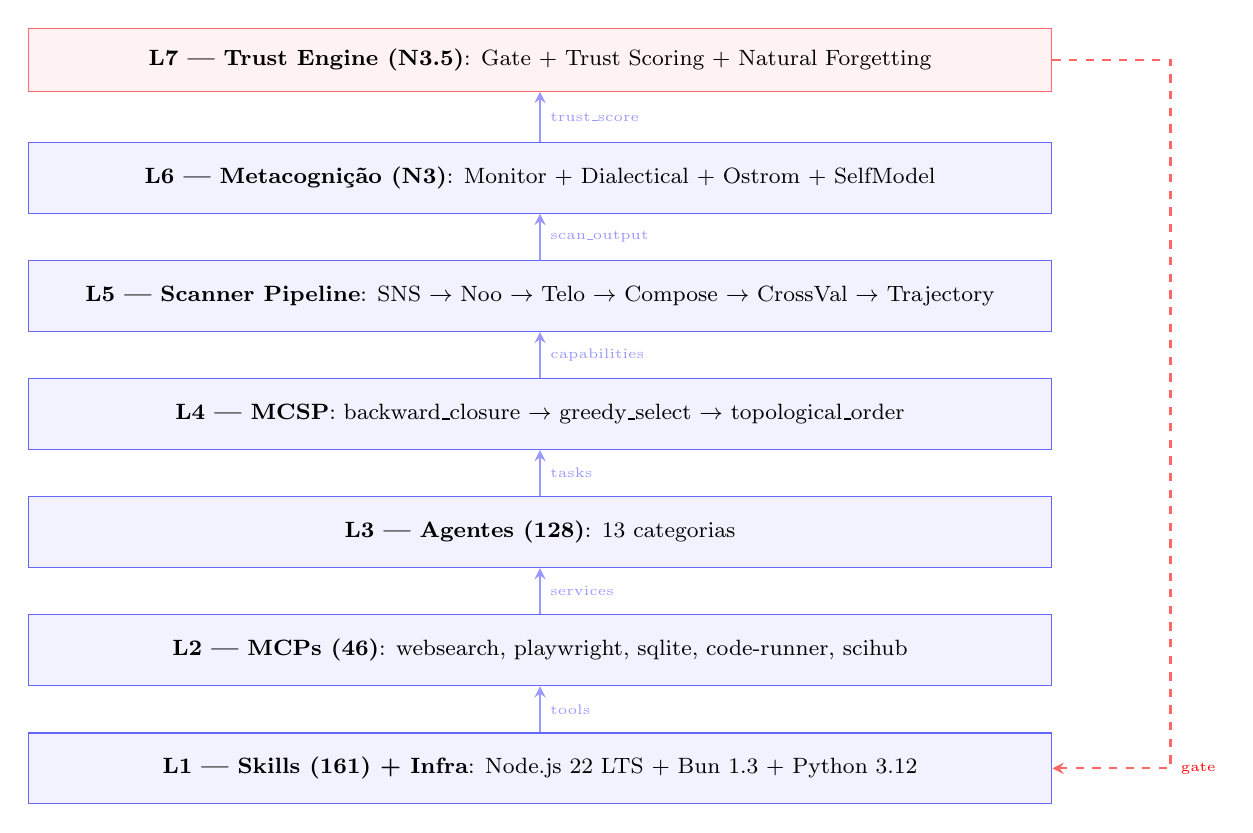
\begin{tikzpicture}[
    layer/.style={rectangle, draw=blue!60, fill=blue!5, minimum width=13cm, minimum height=0.9cm, align=center, font=\footnotesize},
    arrow/.style={->, >=stealth, thick, blue!40},
    gate/.style={rectangle, draw=red!60, fill=red!5, minimum width=13cm, minimum height=0.8cm, align=center, font=\footnotesize},
]
\node[gate] (L7) at (0,6.5) {\textbf{L7 — Trust Engine (N3.5)}: Gate + Trust Scoring + Natural Forgetting};
\node[layer] (L6) at (0,5) {\textbf{L6 — Metacognição (N3)}: Monitor + Dialectical + Ostrom + SelfModel};
\node[layer] (L5) at (0,3.5) {\textbf{L5 — Scanner Pipeline}: SNS $\rightarrow$ Noo $\rightarrow$ Telo $\rightarrow$ Compose $\rightarrow$ CrossVal $\rightarrow$ Trajectory};
\node[layer] (L4) at (0,2) {\textbf{L4 — MCSP}: backward\_closure $\rightarrow$ greedy\_select $\rightarrow$ topological\_order};
\node[layer] (L3) at (0,0.5) {\textbf{L3 — Agentes (128)}: 13 categorias};
\node[layer] (L2) at (0,-1) {\textbf{L2 — MCPs (46)}: websearch, playwright, sqlite, code-runner, scihub};
\node[layer] (L1) at (0,-2.5) {\textbf{L1 — Skills (161) + Infra}: Node.js 22 LTS + Bun 1.3 + Python 3.12};

\draw[arrow] (L1.north) -- (L2.south) node[midway,right,font=\tiny] {tools};
\draw[arrow] (L2.north) -- (L3.south) node[midway,right,font=\tiny] {services};
\draw[arrow] (L3.north) -- (L4.south) node[midway,right,font=\tiny] {tasks};
\draw[arrow] (L4.north) -- (L5.south) node[midway,right,font=\tiny] {capabilities};
\draw[arrow] (L5.north) -- (L6.south) node[midway,right,font=\tiny] {scan\_output};
\draw[arrow] (L6.north) -- (L7.south) node[midway,right,font=\tiny] {trust\_score};
\draw[arrow, red!60, dashed] (L7.east) -- ++(1.5,0) |- (L1.east) node[midway,right,font=\tiny,red] {gate};
\end{tikzpicture}%
}
\caption{Arquitetura do OpenCode Ecosystem — 7 Camadas com Fluxo de Dados}
\label{fig:arquitetura}
\end{figure}

A Figura~\ref{fig:arquitetura} ilustra a arquitetura em 7 camadas. O fluxo de dados é ascendente: Skills (L1) fornecem conhecimento, MCPs (L2) proveem ferramentas, Agentes (L3) executam tarefas. O MCSP (L4) encontra o conjunto mínimo de capacidades. O Scanner Pipeline (L5) diagnostica gaps. A Metacognição (L6) observa, detecta e corrige. O Trust Engine (L7) atua como gate preventivo — a seta tracejada vermelha mostra o ciclo de feedback: após cada execução, o outcome atualiza o trust score, que influencia a próxima decisão do gate.
